\documentclass{article}

\usepackage[preprint]{tmlr}

\usepackage{amsmath,amssymb,amsthm}
\usepackage{booktabs}
\usepackage{graphicx}
\usepackage{xcolor}
\usepackage{multirow}
\usepackage{hyperref}

\newtheorem{proposition}{Proposition}

\renewcommand{\arraystretch}{1.3}

\title{When Site-Level Averages Mislead:\\Two Failure Modes of Ecological Bias in Federated COVID-19 Analysis}

\author{\name Elliot Tower \\
      \email elliot@elliottower.ai}

\begin{document}
\maketitle

\begin{abstract}
Multi-site medical studies and federated analysis networks routinely pool
site-level summaries to draw conclusions about individual patients.  We test
this practice using 42 million individual COVID-19 patient records and
identify two failure modes of ecological bias.

\textbf{Failure mode 1: the signal disappears.}  Using 38 million CDC
records partitioned into 9 demographic pseudo-sites, site-level regression
cannot detect the relationship between age and mortality ($\beta = +0.28$,
$p = 0.12$), while individual-level analysis finds that patients over 80
have 9.9 times the odds of dying ($p < 10^{-300}$).

\textbf{Failure mode 2: the signal distorts.}  Using 4 million confirmed
COVID-19 cases across Mexico's 32 states---real geographic sites---site-level
regression detects a significant relationship ($\beta = +1.31$,
$p < 0.0001$, $R^2 = 0.50$), but the ecological effect size bears no
resemblance to the individual-level truth (age 70+ OR $= 11.3$).

These failures have clinical consequences.  Applied to the 4CE consortium's
22,000-patient neurological COVID-19 dataset (21 hospitals, 6 countries),
meta-analytic methods diverge by 350-fold on the pooled effect
($I^2 = 99.8\%$), the proportion of elderly patients explains most
between-site variation ($\beta = +14.2$, $p < 10^{-15}$), and a
multivariate consistency test detects coordinated cross-site heterogeneity
in comorbidity correlations ($z = 25$, $p < 0.0001$) that standard tests
miss entirely.  Per-site interaction analyses on all three datasets
show that the age--comorbidity relationship varies across sites (CDC:
2-fold; Mexico: 2-fold; 4CE: age $\times$ mortality $p < 0.04$ at all
timepoints), confirming that pooling loses information about effect
modification.  Two datasets, two failure modes.  The implication for federated
networks is blunt: a pooled site-level summary is a hypothesis, not a
finding---test it on individual patients before acting on it.
\end{abstract}


\section{Introduction}

Suppose ten hospitals each report the fraction of their COVID-19 patients who
died.  A meta-analysis averages those fractions and reports the result as
``the'' mortality rate.  The same logic underlies federated analysis
networks such as ENACT, TriNetX, and PCORnet, where hospitals share summary
statistics rather than individual records.  This approach works when the
hospitals are measuring the same thing in the same kind of patient.

They rarely are.

Hospitals differ in who walks through the door.  One serves a young urban
population; another, a rural elderly community.  One codes aggressively for
neurological complications; another barely records them.  The average across
these hospitals is a real number, but it may not describe any actual hospital
or any actual patient.  Worse, it can point in the wrong direction entirely.

This problem---drawing conclusions about individuals from group-level
data---is the \emph{ecological fallacy}
\cite{robinson1950ecological}.  The structural mechanisms behind it---aggregation
bias, cross-level confounding, and specification error---are well understood
\cite{greenland1992ecological,greenland2001ecologic}.
Known since 1950 and taught in every
epidemiology course, it is routinely acknowledged and routinely ignored.
Multi-site consortium studies and federated analysis networks typically have
access only to site-level summaries and treat them as proxies for
patient-level truth.

We test how badly this matters using 42 million individual COVID-19 patient
records from two countries, plus a third dataset of 22,000 patients from 21
hospitals across 6 countries.  The CDC dataset uses race/ethnicity categories
as pseudo-sites---an intentionally extreme grouping that maximizes
compositional confounding.  Mexico's 32 states provide a confirmatory test
on real geographic sites with less extreme demographic variation.  Together
the two datasets bracket the severity range: the CDC shows ecological bias
at its worst, and Mexico shows that real administrative units do not escape
it.  The gap between site-level and individual-level analysis is large in
both cases.  We find two failure modes:

\begin{enumerate}
\item \textbf{The signal disappears.}  Site-level analysis of 38 million CDC
records cannot detect the relationship between age and mortality
($p = 0.12$).  Individual-level analysis finds a 9.9-fold odds ratio
($p < 10^{-300}$).

\item \textbf{The signal distorts.}  Site-level analysis of 4 million
Mexican COVID-19 records finds a significant relationship
($p < 0.0001$), but the ecological effect size ($\beta = +1.31$) bears no
resemblance to the individual-level truth (OR $= 11.3$).  The regression
reports a linear slope; the patient-level reality is a multiplicative odds
ratio an order of magnitude larger.
\end{enumerate}

We then ask: if federated networks are constrained to site-level summaries,
can anything be done?  We show that structural consistency tests---methods
that examine the \emph{structure} of relationships across sites, rather than
averaging over them---can diagnose when site-level pooling is unreliable.
Applied to the 4CE consortium's neurological COVID-19 dataset, these methods
detect coordinated heterogeneity invisible to standard meta-analysis.  When
site-level averages fail in two different ways on two different datasets,
federated analyses should treat their pooled summaries as hypotheses for
individual-level testing.


\section{Ecological Bias: Two Failure Modes}

\subsection{Failure mode 1: the signal disappears (CDC, United States)}

We start with the simplest possible question: does age predict COVID-19
mortality?  The answer is obviously yes.  The question is whether site-level
analysis can find it.

The CDC Case Surveillance dataset contains 38.2 million confirmed COVID-19
cases with age group, sex, race/ethnicity, hospitalization status, ICU
admission, and death.  We used race/ethnicity categories as pseudo-sites (9
groups with $n \geq 1{,}000$), mimicking what a consortium study would have
if each racial/ethnic group were a separate hospital reporting summary
statistics.  This is a deliberate simplification that maximizes
compositional confounding; the specific confounders differ from those in
hospital-based consortia (see Limitations).

\textbf{Site-level analysis} aggregated each group's mortality rate
(deaths/cases) and proportion of patients aged 80+, then regressed one on the
other across the 9 groups.  Result: no significant relationship ($\beta =
+0.28$ mortality-rate units per unit proportion elderly, $p = 0.12$,
$R^2 = 0.31$).  A 10-percentage-point increase in the elderly share is
associated with a 2.8-percentage-point increase in the group mortality
rate---but this association is not distinguishable from noise.  Site-level
analysis cannot detect that age predicts mortality.

\textbf{Individual-level analysis} on the same 38.2 million patients found
that being over 80 multiplies the odds of death by 9.9 ($p < 10^{-300}$).
After adjusting for sex and comorbidities, patients gain 2.4 times the odds of
dying for each additional decade of age ($p < 10^{-300}$).  Males have 1.7
times the odds; patients with underlying conditions have 1.5 times the odds.

The effect is unambiguous at the individual level and invisible at the site
level (Figure~\ref{fig:ecological}A).  This is the ecological fallacy at its most extreme.  The effect
isn't distorted---it's gone.


\subsection{Failure mode 2: the signal distorts (Mexico)}

The CDC demonstration uses pseudo-sites (racial/ethnic groups), which one
might dismiss as an artifact of the grouping choice.  Mexico's COVID-19
surveillance data provides a stronger test: 3,993,464 confirmed cases across
32 real geographic states, each corresponding to the state of the treating
medical unit.

\textbf{Site-level analysis} across the 32 states finds a significant
relationship between the proportion of patients aged 70+ and the state
mortality rate ($\beta = +1.31$ mortality-rate units per unit proportion
elderly, $p < 0.0001$, $R^2 = 0.50$).  Concretely, a 10-percentage-point
increase in a state's elderly share predicts a 13.1-percentage-point
increase in state mortality.  The ecological regression
``works''---it detects a real signal, unlike the CDC analysis.

\textbf{Individual-level analysis} on the same 4 million patients reveals the
true effect: patients aged 70 or older have 11.3 times the odds of dying
($p < 10^{-300}$).  After adjusting for sex and 9 individual comorbidities
(diabetes, hypertension, obesity, cardiovascular disease, chronic kidney
disease, COPD, asthma, immunosuppression, and smoking), the adjusted odds
ratio remains 8.0 ($p < 10^{-300}$).  Males have 1.7 times the odds;
patients with any comorbidity have 3.8 times the odds.

Site-level analysis gets the direction right and the size wrong (Figure~\ref{fig:ecological}B): a linear
slope of $+1.31$ standing in for an odds ratio of 11.  The two numbers
don't even measure the same kind of thing.

\begin{table}[t]
\centering
\caption{Two failure modes of ecological bias.  The CDC analysis (pseudo-sites)
\emph{misses} the age--mortality relationship entirely.  The Mexico analysis
(real geographic sites) \emph{detects} a relationship but in the wrong
functional form and at the wrong scale.  Individual-level analysis on both
datasets finds large, unambiguous effects.}
\label{tab:ecological}
\begin{tabular}{llcc}
\toprule
Dataset & Analysis level & Effect size & $p$-value \\
\midrule
\multicolumn{4}{l}{\emph{CDC (38.2M cases, 9 pseudo-sites):}} \\
& Site-level regression & $\beta = +0.28$ & 0.12 \\
& Individual: age per decade & OR $= 2.40$ & $< 10^{-300}$ \\
& Individual: age 80+ & OR $= 9.88$ & $< 10^{-300}$ \\
\midrule
\multicolumn{4}{l}{\emph{Mexico (4.0M cases, 32 states):}} \\
& Site-level regression & $\beta = +1.31$ & $< 0.0001$ \\
& Individual: age 70+ & OR $= 11.26$ & $< 10^{-300}$ \\
& Individual: adjusted & OR $= 7.97$ & $< 10^{-300}$ \\
\bottomrule
\end{tabular}
\end{table}

\begin{figure}[t]
\centering
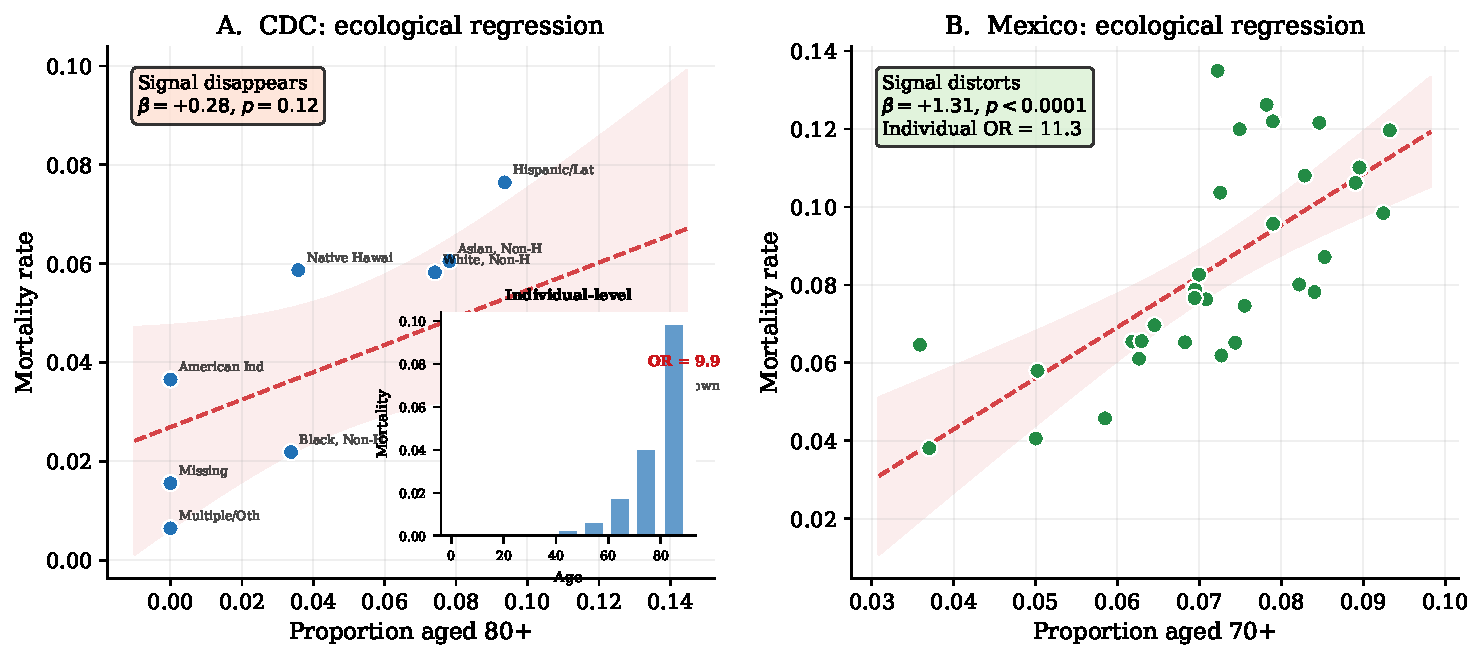
\includegraphics[width=\textwidth]{figures/fig1_ecological_bias.pdf}
\caption{Site-level ecological regressions for the two datasets.
\textbf{(A)}~CDC: 9 race/ethnicity pseudo-sites show no significant relationship
between the proportion of elderly patients and site mortality
($\beta = +0.28$, $p = 0.12$), despite a 9.9-fold individual-level odds ratio.
\textbf{(B)}~Mexico: 32 states show a significant ecological slope
($\beta = +1.31$, $p < 0.0001$), but this linear coefficient is
incommensurable with the individual-level odds ratio of 11.3.
Panel~A illustrates signal disappearance; Panel~B illustrates signal distortion.}
\label{fig:ecological}
\end{figure}

These two failure modes are complementary.  The CDC data shows that
ecological analysis can miss a 9.9-fold odds ratio entirely.  The Mexico
data shows that even when ecological analysis detects a signal, it reports
a linear slope where the patient-level truth is a multiplicative odds ratio
11 times the baseline---a different quantity, not a noisy estimate of the
same one.  Any federated analysis relying on site-level summaries faces
both risks simultaneously.


\subsection{Why does this happen?}

The ecological fallacy arises from confounding at the group level.  To see
the mechanism, consider the CDC data.

The group with the highest proportion of 80+ patients (``Unknown'' race,
13.5\%) has lower mortality (3.3\%) than the group with the second-highest
elderly proportion (Hispanic, 9.4\%, mortality 7.6\%), because the Unknown
group has different sex composition and comorbidity rates.  Groups also
differ in sex ratios (15\% to 65\% male) and comorbidity prevalence (0.5\%
to 14\%).  These differences scramble the age--mortality relationship at the
group level.

At the individual level, confounders are controlled directly: the logistic
regression asks ``among patients with the same sex and comorbidity status,
does age predict death?''  The answer is unambiguous.

Mexico illustrates the second mechanism.  The 32 states have less extreme
compositional variation than the CDC pseudo-sites (the states are real
geographic units, not demographic slices), so the ecological regression does
detect a directional signal.  The distortion arises from aggregation bias:
the regression fits a linear slope to state-level proportions, while the
true patient-level relationship is a nonlinear odds ratio.  Simpson's
paradox does not apply in the classic sense---the direction is preserved---but
the magnitude and functional form are lost entirely.

Any federated analysis reporting pooled site-level averages could therefore
be reporting the wrong magnitude, the wrong functional form, or no effect
at all---depending on the confounding structure of the network's sites.

\paragraph{A note on effect sizes.}
This paper reports several quantities that share the name ``effect size''
but measure different things.  Ecological regression coefficients ($\beta$)
are linear slopes across site-level proportions.  Individual-level odds
ratios (OR) are multiplicative risk comparisons within patients.
Proportional morbidity indices (PMI) are ratios of observed to expected
disease counts.  These quantities are not comparable: a $\beta$ of $+1.31$
and an OR of $11.3$ describe the same underlying relationship at different
levels of analysis and in different functional forms.  This
incommensurability is itself the point---ecological analysis does not
produce a noisy estimate of the patient-level effect; it produces a
different quantity entirely.


\section{Clinical Consequences: The 4CE Neurological Dataset}

The ecological bias demonstrated in Sections~2.1--2.2 has direct clinical
consequences.  The 4CE consortium (Consortium for Clinical Characterization
of COVID-19 by EHR) analyzed neurological outcomes in over 22,000
hospitalized patients across 21 hospitals in 6 countries
\cite{four_ce_neuro2021}, using only aggregate site-level data.  We
re-analyze this dataset to show that its pooled estimates are unreliable
in the ways the ecological fallacy predicts.


\subsection{CNS involvement and the 350-fold method divergence}

Among well-measured sites ($\text{SE} < 0.5$ on the log scale; $k = 11$--16
per timepoint), the fixed-effects proportional morbidity index (PMI) for CNS
involvement is 1.97 (95\% CI: [1.87, 2.09]) at 30 days.  This estimate must
be interpreted cautiously: $I^2 = 99.8\%$ (Cochran's $Q = 6318$, $p <
10^{-15}$) means essentially all variation is between-site, violating the
common-effect assumption that fixed-effects requires.

The 350-fold divergence between pooling methods (Table~\ref{tab:meta}) is a
diagnostic failure.  The random-effects PMI of 702 is a numerical artifact:
several small sites produce PMIs of $10^{8}$--$10^{18}$ from complete
separation, and the random-effects framework up-weights these extreme
estimates.  Among the 11 sites with $\text{SE} < 0.4$, the picture is more
consistent (PMIs between 1.4 and 2.8), but even this restricted set shows
$I^2 > 95\%$.  The method divergence signals that this dataset requires
decomposition of heterogeneity rather than a pooled estimate.

\begin{table}[t]
\centering
\caption{\textbf{The 350-fold divergence between pooling methods is a
diagnostic artifact, not a finding.}  The random-effects PMI of 702 results
from complete separation at small sites (PMIs of $10^{8}$--$10^{18}$)
up-weighted by the DerSimonian--Laird estimator.  No single pooled number
is appropriate for this data ($I^2 = 99.8\%$).  The divergence itself is
the result: it signals that the underlying heterogeneity requires
decomposition, not averaging.}
\label{tab:meta}
\begin{tabular}{llccc}
\toprule
Method & Pooled PMI & 95\% CI & $p$ & $I^2$ \\
\midrule
Fixed-effects (IV) & 1.97 & [1.87, 2.09] & $< 10^{-6}$ & 99.8\% \\
Random-effects (DL) & 702 & [201, 2460] & $< 10^{-6}$ & --- \\
Influence function & 972 & [1.6, 587K] & 0.035 & --- \\
\bottomrule
\end{tabular}
\end{table}

Peripheral nervous system involvement provides a negative control.  PNS
diagnoses show a PMI of 1.04 at 30 days (95\% CI: [0.95, 1.14],
$p = 0.37$), indistinguishable from the null.  If the CNS effect were
driven by sicker patients receiving more diagnostic workups (which would
also detect peripheral neuropathies), PNS diagnoses should show a similar
signal.  They do not.  The specificity to CNS involvement is consistent
with SARS-CoV-2 neuroinvasion through the blood-brain barrier
\cite{song2021neuroinvasion} and central neuroinflammation
\cite{iadecola2020covid}, mechanisms that do not produce peripheral
neuropathy.


\subsection{Age drives between-site variation}

Meta-regression of the CNS severity effect (30-day PMI, log scale) on four
site-level demographics identifies the proportion of elderly patients as the
strongest moderator ($\beta = +14.2$, $\text{SE} = 0.83$,
$p < 10^{-15}$).  The direction is clear: sites serving older populations
show larger neurological effects.  The magnitude should be treated as
directional evidence only.  With ${\sim}20$ sites, Type~M error
\cite{gelman2014typeMS} systematically inflates significant coefficients;
hierarchical shrinkage is the appropriate estimator for effect size, and
we report $\beta = +14.2$ as evidence that elderly proportion is the
dominant moderator, not as an estimate of its strength.

This pattern is consistent with age-dependent blood-brain barrier
vulnerability \cite{montagne2015bbb} and chronic low-grade inflammation
\cite{franceschi2018inflammaging}, but site-level data cannot distinguish
this biological explanation from compositional confounding: sites with more
elderly patients also differ in comorbidity burden, coding practices, and
clinical management.

\begin{table}[t]
\centering
\caption{Meta-regression moderators of the CNS severity association (30-day
PMI).  Elderly proportion is the strongest moderator.  Baseline severity
acts in the opposite direction (ceiling effect).  The large $\beta$
magnitudes are likely inflated by Type~M error \cite{gelman2014typeMS} from
$\sim$20 sites.}
\label{tab:moderators}
\begin{tabular}{lcccc}
\toprule
Moderator & $\beta$ & SE & $p$ & Range across sites \\
\midrule
Proportion age $\geq 80$ & $+14.2$ & 0.83 & $< 10^{-15}$ & 0.01--0.43 \\
Proportion female & $+1.13$ & 0.14 & $< 10^{-15}$ & 0.06--0.53 \\
Baseline severity & $-2.91$ & 0.23 & $< 10^{-15}$ & 0.06--0.73 \\
Number of patients & $-0.0003$ & 0.00005 & $< 10^{-9}$ & 32--22{,}789 \\
\bottomrule
\end{tabular}
\end{table}

A site-level interaction between elderly proportion and mortality rate is
significant at all three follow-up periods ($p < 0.04$ uncorrected),
increasing from 30 to 90 days ($\beta$: $+32.5 \to +38.3$), though the
temporal trend itself has only three timepoints and does not reach
significance ($p = 0.16$).  Under Benjamini--Hochberg FDR control across the
18-test interaction family (6 covariate pairs $\times$ 3 timepoints),
only the 60-day ($p = 0.024$) and 90-day ($p = 0.021$) age--mortality
interactions survive; the 30-day value ($p = 0.037$) does not.  The
coefficient magnitudes ($\beta = +32$ to $+38$) are directional evidence
only: estimated from ${\sim}20$ aggregated sites, they are characteristic
of Type~M inflation \cite{gelman2014typeMS} and should not be interpreted
as effect sizes.  Hierarchical meta-regression with site random effects
\cite{gelman2012multilevel} would shrink these toward the group mean;
the shrinkage factor $\hat\tau^2 / (\hat\tau^2 + \hat\sigma_i^2)$ is
likely substantial given the small number of sites and high between-site
variance.


\subsection{Comorbidity correlations differ systematically across sites}

Elixhauser comorbidity correlation matrices \cite{elixhauser1998} from 20
4CE sites show collective inconsistency when tested with a multivariate
consistency statistic: $z = 25.0$ ($p < 0.0001$), with comparable signals
in CNS-only ($z = 14.4$) and PNS-only ($z = 14.4$) subgroups
(Table~\ref{tab:consistency}).

\begin{table}[t]
\centering
\caption{Cross-site consistency of comorbidity correlation patterns.  The
multivariate consistency statistic detects collective inconsistency
($z = 25$) that pairwise Cochran's $Q$ tests miss entirely (0/1305
significant).}
\label{tab:consistency}
\begin{tabular}{lccc}
\toprule
Test & Statistic & $p$ & Significant pairs \\
\midrule
Consistency (all patients) & $z = 25.0$ & $< 0.0001$ & N/A (collective) \\
Consistency (CNS only) & $z = 14.4$ & $< 0.0001$ & N/A (collective) \\
Consistency (PNS only) & $z = 14.4$ & $< 0.0001$ & N/A (collective) \\
Cochran's $Q$ (per pair) & max $Q = 13.4$ & all $> 0.05$ & 0/1305 \\
\bottomrule
\end{tabular}
\end{table}

No single comorbidity pair varies enough across sites to reach significance
on its own.  The consistency test detects their collective pattern: the
aggregate structure of small per-pair differences is far more extreme than
chance.  Standard meta-analysis assumes the covariate relationships being
adjusted for are constant across sites; this result says they are not.  The most
heterogeneous pairs---HIV-Lymphoma ($Q = 13.4$, $r = 0.09 \pm 0.25$) and
Alcohol-Drugs ($Q = 12.9$, $r = 0.70 \pm 0.24$)---illustrate how coding
and documentation practices drive cross-site inconsistency that the
collective test detects.


\section{Structural Diagnostics Across All Three Datasets}

When individual data is unavailable, can federated networks diagnose
whether their site-level summaries are trustworthy?  Two structural
diagnostics---the consistency statistic and per-site interaction
analysis---provide partial answers.

\subsection{The consistency test: power requires heterogeneous coverage}

The consistency statistic measures whether per-site correlation matrices
disagree more than expected by chance.  Its power depends on a structural
property of the data: whether different sites report different subsets of
variable pairs (heterogeneous coverage) or all report the same pairs
(homogeneous coverage).

On the CDC data (9 groups, all reporting all 15 variable pairs), the
permutation null is degenerate: $z = 0$, null standard deviation
$< 10^{-16}$.  On Mexico's 32 states (all reporting all 15 pairs), the
same degeneracy appears: $z = 0.47$, effectively null.
Appendix~\ref{app:degeneracy} proves this is a mathematical necessity:
within-dimension permutation preserves the test statistic when coverage is
homogeneous.

On the 4CE data, where coverage is heterogeneous (10 sites report
36--296 of 1,305 possible comorbidity pairs; 10 report all 1,305), the
same test produces $z = 25$ ($p < 0.0001$).  The test's power depends on
heterogeneous coverage---a property of the data structure, not the signal.
This is a practical guide for federated networks: the consistency test is
most useful when sites have different measurement capabilities,
which is the norm in multi-national consortia.


\subsection{Per-site interactions: effect modification varies everywhere}

Per-site logistic regressions reveal genuine variation in the
age $\times$ comorbidity interaction across all three datasets.

\textbf{CDC (9 pseudo-sites).}  All groups show that comorbidity matters
less in the elderly (all interaction OR $< 1$), but the magnitude varies
3-fold: from OR $= 0.23$ (Missing) to OR $= 0.69$ (Hispanic/Latino), all
significant ($p < 10^{-4}$).  Dropping the two groups with ambiguous
demographic composition (Unknown and Missing) leaves 7 groups spanning
0.27--0.69, a 2.6-fold range.  The pooled individual-level regression
confirms the interaction is real (OR $= 0.92$ per decade,
$p < 10^{-132}$).

\textbf{Mexico (32 states).}  The same pattern holds with real geographic
sites: pooled interaction OR $= 0.32$ ($p < 10^{-300}$), with per-state
values ranging from 0.19 (Quintana Roo) to 0.38 (Mexico City), a 2-fold
range.  All 32 states show sub-additive interactions---comorbidity adds
less mortality risk in the elderly---but the magnitude of this attenuation
varies by state.

\textbf{4CE (21 hospitals).}  The age $\times$ mortality interaction on the
neurological severity effect is significant at all three timepoints
($p < 0.04$ uncorrected), with coefficients that increase from
$\beta = +32.5$ at 30 days to $\beta = +38.3$ at 90 days.

The consistency of per-site interaction variation across three independent
datasets---with different countries, different site definitions, and
different outcome measures---is direct evidence that pooling the
age--comorbidity or age--mortality relationship across sites loses
information about effect modification.

\begin{table}[t]
\centering
\caption{Summary of methods applied across all three datasets.  The
consistency statistic has power only on heterogeneous-coverage data (4CE).
Per-site interaction analysis detects effect modification on all three
datasets.  Individual-level analysis (where available) gives the true
answer.}
\label{tab:comparison}
\begin{tabular}{llcc}
\toprule
Method & Dataset & Statistic & $p$ \\
\midrule
\multirow{3}{*}{Ecological regression}
  & CDC (9 groups) & $\beta = +0.28$ & 0.12 \\
  & Mexico (32 states) & $\beta = +1.31$ & $< 0.0001$ \\
  & 4CE (21 hospitals) & PMI $= 2.0$ & $< 10^{-6}$ \\
\midrule
\multirow{3}{*}{Consistency statistic}
  & CDC & degenerate & --- \\
  & Mexico & degenerate & --- \\
  & 4CE & $z = 25$ & $< 0.0001$ \\
\midrule
\multirow{3}{*}{Per-site interaction}
  & CDC & OR: 0.23--0.69 & all $< 10^{-4}$ \\
  & Mexico & OR: 0.19--0.38 & all $< 10^{-4}$ \\
  & 4CE & $\beta$: $+32$ to $+38$ & $< 0.04$ \\
\midrule
\multirow{2}{*}{Individual logistic}
  & CDC & OR $= 9.88$ & $< 10^{-300}$ \\
  & Mexico & OR $= 11.26$ & $< 10^{-300}$ \\
\bottomrule
\end{tabular}
\end{table}


\section{Discussion}

\subsection{Two failure modes, one underlying problem}

Ecological bias in federated studies fails in two ways, depending on the
confounding structure of the network's sites.

In the CDC data, where race/ethnicity groups differ sharply in sex and
comorbidity composition, the ecological regression cannot detect an
individual-level odds ratio of 9.9.  The signal vanishes entirely---a
false negative.  In the Mexico data, where the 32 states have more
homogeneous demographics, the ecological regression does detect a
directional signal, but reports it as a linear slope of $+1.31$ where the
patient-level truth is a multiplicative odds ratio of 11.  The false
negative is the more obvious danger.  The distorted positive may be worse
in practice: it looks like confirmation, and the number it produces is
meaningless.

Underneath both is the same mechanism: aggregation destroys the within-site
covariance structure that individual-level analysis exploits.  For
federated networks such as ENACT, TriNetX, and PCORnet, the implication
is direct: site-level summaries should never be treated as sufficient
statistics for the patient-level relationships they purport to represent.

\subsection{Implications for federated causal discovery}

Federated analysis networks face a structural tension.  Privacy
constraints and data governance restrict them to site-level summaries, but
ecological bias means these summaries can miss or distort patient-level
effects.  The consistency test and per-site interaction
analysis offer partial diagnostics: the consistency test detects
coordinated heterogeneity when coverage is heterogeneous, and per-site
interaction analysis detects effect modification regardless of coverage
structure.

Neither tool recovers the individual-level answer; both only flag that
site-level pooling is unreliable.  Three approaches go further:

\textbf{Federated regression.}  Sites run a standardized analysis script
locally and share only coefficients (point estimates, standard errors, and
sample sizes).  This preserves patient privacy while enabling
individual-level estimation via meta-analysis of patient-level effects
rather than meta-analysis of ecological summaries.  Implementations already
exist: Fed-GLMM~\cite{chen2023fedglmm} achieves near-identical results to
pooled generalized linear mixed models while sharing only summary statistics,
and DataSHIELD~\cite{wilson2022datashield} provides privacy-preserving
survival analysis across federated nodes.

\textbf{Large individual-level cohorts.}  N3C~\cite{haendel2021n3c}
(15 million patients, 75+ hospital sites, full EHR) and ISARIC (705,000
hospitalized patients, 1,500+ sites, 60 countries) contain the individual
records needed to directly test whether neurological involvement predicts
severity after patient-level adjustment.

\textbf{Hierarchical models with site random effects.}  As
Diez-Roux~\cite{diezroux2000multilevel} and
Subramanian et al.~\cite{subramanian2009revisiting} argued, neither
purely ecological nor purely individualistic analysis suffices---what is
needed is multilevel models incorporating both levels.  When
individual-level data is available, a hierarchical model with site as a
random intercept directly addresses both the ecological fallacy (by
estimating patient-level effects) and the Type~M inflation problem (by
shrinking extreme site-level estimates toward the group mean
\cite{gelman2012multilevel}).  The shrinkage factor is approximately
$\hat\tau^2 / (\hat\tau^2 + \hat\sigma_i^2)$, where $\hat\tau^2$ is
the between-site variance and $\hat\sigma_i^2$ is the within-site
sampling variance.

\subsection{Practical guidelines for multi-site studies}

The ecological fallacy is not specific to COVID-19.  Any multi-site
study---genome-wide association, multi-center drug trials, educational
interventions---faces the same risk when the units of analysis (sites)
differ systematically from the units of inference (people).

Our results point to three lessons.  First, report heterogeneity honestly:
$I^2 = 99.8\%$ means the pooled average is almost meaningless, and the
full distribution of site-level effects should appear alongside it.
Second, test the structure, not just the average.  Consistency tests detect
coordinated between-site differences that Cochran's $Q$ (one variable at a
time) and geometric distance methods (expected demographic variation) both
miss; hierarchical models with site random effects address both the
multiplicity problem (through partial pooling) and Type~M inflation
(through shrinkage).  Third, seek individual data.  The ecological fallacy
is a problem of aggregation; the only definitive solution is
disaggregation, and modern frameworks---federated regression, secure
enclaves, synthetic data---make this feasible even when raw records cannot
leave the hospital.  Throughout, disclose the full analysis menu: state how
many tests were run and report all results, including nulls.


\section{Methods}

\subsection{Data sources}

\textbf{CDC Case Surveillance.}  The CDC COVID-19 Case Surveillance Public
Use Dataset contains 38,173,454 confirmed and probable COVID-19 cases reported
to the CDC through 2022.  Each record includes onset date, age group (9
categories: 0--9 through 80+), sex, race/ethnicity (9 categories),
hospitalization, ICU admission, death, and underlying medical condition (binary
flag).  No geographic identifiers are present in the public version.  We used
race/ethnicity categories as pseudo-sites, restricted to groups with $n \geq
1{,}000$ (9 groups, $n$ ranging from 13,548 to 6,165,036).

\textbf{Mexico Datos Abiertos.}  Mexico's Secretar\'{i}a de Salud publishes
individual-level COVID-19 surveillance data covering all confirmed and
suspected cases nationwide.  We used the January 3, 2022 historical snapshot
(12,425,179 total records, 3,993,464 confirmed COVID-19 cases, 299,581
deaths).  Each record includes age, sex, state of the treating medical unit
(ENTIDAD\_UM, 32 states), death date, and 9 individual comorbidity flags
(diabetes, hypertension, obesity, cardiovascular disease, chronic kidney
disease, COPD, asthma, immunosuppression, smoking).  Cases were classified as
confirmed when CLASIFICACION\_FINAL $\in \{1, 2, 3\}$.  We used state of
medical unit as the site variable, providing 32 real geographic sites with
$n$ ranging from 8,759 (Colima) to 637,408 (Mexico City).

\textbf{4CE Consortium.}  Aggregate site-level data from the 4CE consortium's
Phase 2.1 Neurological Analysis \cite{four_ce_neuro2021}: 21 healthcare sites
across 6 countries (USA, France, Germany, UK, Singapore, Italy), over 22,000
hospitalized COVID-19 patients.  Data included site-level demographics,
Elixhauser comorbidity scores \cite{elixhauser1998}, and proportional morbidity
index (PMI) for CNS and PNS neurological involvement at 30, 60, and 90 days.

\subsection{Statistical analyses}

\textbf{Ecological regression.}  For each dataset, we computed per-site
proportions of elderly patients and mortality rates, then regressed site
mortality on site elderly proportion using ordinary least squares.  For CDC
data, elderly was defined as age 80+; for Mexico, age 70+.

\textbf{Individual-level logistic regression.}  We fit logistic regression
models on the complete individual-level data: (1)~death $\sim$ age;
(2)~death $\sim$ age + sex + comorbidity; (3)~death $\sim$ age $\times$
comorbidity + sex.  For the CDC data, age was coded as the midpoint of the
age group (5, 15, \ldots, 85); for Mexico, age was continuous, dichotomized
at 70.  Odds ratios are reported per decade (CDC) or as binary contrasts
(Mexico).  We used \texttt{statsmodels} v0.14 for estimation.

\textbf{Per-site interaction analysis.}  For each site in each dataset, we
fit a logistic regression with an age $\times$ comorbidity interaction term.
For the 4CE data (no individual records), we fit weighted meta-regressions
with interaction terms on site-level demographics.

\textbf{Multivariate consistency test.}  We computed per-site Pearson
correlation matrices (6 binary variables for CDC and Mexico; 30 Elixhauser
comorbidity categories for 4CE) and measured global consistency as the mean
sum of squared pairwise differences across all site pairs, normalized by
shared coverage.  Significance was assessed by 500 within-dimension
permutations.  The test's power depends on heterogeneous coverage
(Appendix~\ref{app:degeneracy}).

\textbf{4CE meta-analysis.}  Per-site log-PMI estimates were pooled using
fixed-effects (inverse-variance), DerSimonian--Laird random-effects, and
influence-function methods.  Sites with $\text{SE} \geq 0.5$ were excluded
from primary analyses.  Meta-regression of log-PMI on four site-level
demographics used weighted least squares.  E-values \cite{vanderweele2017}
assess sensitivity to unmeasured confounding.

\subsection{Multiple testing}

Table~\ref{tab:multiplicity} enumerates all hypothesis tests reported in
the paper.  Five are pre-specified primary analyses: the ecological
regression and individual-level logistic regression on CDC and Mexico data,
plus the 4CE fixed-effects PMI.  Twelve additional 4CE analyses are
secondary or exploratory: meta-regression moderators (4), consistency
tests (3), interaction tests at three timepoints (3), the PNS negative
control (1), and the temporal trend across timepoints (1).
Benjamini--Hochberg FDR correction at $q = 0.05$ was applied within
the 18-test interaction family (6 covariate pairs $\times$ 3
timepoints); of the 3 age--mortality interaction tests, only the 60-
and 90-day values survive correction.  All null results (PNS PMI
$= 1.04$; consistency test degenerate on CDC and Mexico; temporal trend
$p = 0.16$) are reported.

\begin{table}[t]
\centering
\caption{Multiple testing accounting.  Pre-specified tests are the five
primary analyses.  BH-FDR was applied within the 18-test interaction
family (6 covariate pairs $\times$ 3 timepoints); the age--mortality
results shown here are 3 of those 18.}
\label{tab:multiplicity}
\small
\begin{tabular}{llcl}
\toprule
Dataset & Test & $p$ & Status \\
\midrule
CDC & Ecological regression & 0.12 & Pre-specified \\
CDC & Individual logistic (age 80+) & $< 10^{-300}$ & Pre-specified \\
Mexico & Ecological regression & $5.3 \times 10^{-6}$ & Pre-specified \\
Mexico & Individual logistic (age 70+) & $< 10^{-300}$ & Pre-specified \\
4CE & Fixed-effects PMI & $< 10^{-6}$ & Pre-specified \\
\midrule
4CE & Consistency (all patients) & $< 0.0001$ & Secondary \\
4CE & Consistency (CNS only) & $< 0.0001$ & Secondary \\
4CE & Consistency (PNS only) & $< 0.0001$ & Secondary \\
4CE & Meta-regression: elderly & $< 10^{-15}$ & Secondary \\
4CE & Meta-regression: female & $< 10^{-15}$ & Secondary \\
4CE & Meta-regression: severity & $< 10^{-15}$ & Secondary \\
4CE & Meta-regression: N patients & $< 10^{-9}$ & Secondary \\
4CE & Interaction 30-day & 0.037 & Does not survive FDR$^\dagger$ \\
4CE & Interaction 60-day & 0.024 & Survives FDR$^\dagger$ \\
4CE & Interaction 90-day & 0.021 & Survives FDR$^\dagger$ \\
4CE & Temporal trend (30$\to$90 day) & 0.16 & Null \\
4CE & PNS PMI 30-day (negative control) & 0.37 & Null (expected) \\
\bottomrule
\multicolumn{4}{l}{\footnotesize $^\dagger$FDR applied within the
18-test interaction family (6 pairs $\times$ 3 timepoints).}
\end{tabular}
\end{table}

\subsection{Analysis provenance}

The five pre-specified analyses (ecological and individual-level
regressions on CDC and Mexico data; 4CE fixed-effects PMI) were planned
before examining results, following the original 4CE study
protocol~\cite{four_ce_neuro2021}.  All secondary analyses---meta-regression
moderators, site-level interaction tests, the multivariate consistency
test, and PNS negative controls---were developed during exploratory
analysis of the 4CE dataset.  We report all results including nulls
(Table~\ref{tab:multiplicity}).  No analyses were conducted and suppressed.

\subsection{Reproducibility}

All code and analysis scripts will be released on GitHub and archived on
Zenodo upon publication.
The CDC data is publicly downloadable from \texttt{data.cdc.gov} (dataset
\texttt{vbim-akqf}).  The Mexico data is publicly downloadable from
\texttt{datos.gob.mx} (Direcci\'{o}n General de Epidemiolog\'{i}a).


\section{Limitations}

\textbf{Pseudo-sites are not hospitals.}  Race/ethnicity groups in the CDC
data are a proxy for the multi-site structure of consortium studies.  They
differ from hospitals in important ways: they are not geographically
localized, patients within a group may attend different hospitals, and the
grouping confounds race with socioeconomic factors.  The ecological fallacy
demonstration is valid---group-level analysis misses patient-level
effects---but the specific confounders differ from those in a hospital-based
consortium.  The Mexico analysis (32 real geographic sites) partially
addresses this limitation, and the two datasets together bracket the range
of ecological bias severity.

\textbf{Limited variables.}  The CDC public dataset has 12 variables; the
Mexico data has 18.  Hospital-based datasets such as N3C have hundreds.
Our analysis captures the direction of the problem but underestimates its
magnitude: with more variables, the scope for ecological confounding grows.

\textbf{4CE data is aggregate only.}  All 4CE analyses use site-level
summaries.  The ecological fallacy applies directly: site-level associations
need not hold for individual patients, and the age--mortality interaction may
reflect compositional confounding rather than a biological mechanism.  The
age $\times$ mortality interaction coefficients ($\beta = +32$ to $+38$) are
likely inflated by Type~M error from $\sim$20 sites
\cite{gelman2014typeMS}.

\textbf{Consistency tests detect problems, not answers.}  The multivariate
consistency test detects \emph{that} something is wrong with site-level
pooling; it does not tell you \emph{what} the individual-level answer is.
Its power requires heterogeneous coverage---a property present in the 4CE
data but absent in the CDC and Mexico data, where the test is degenerate
(Appendix~\ref{app:degeneracy}).

\textbf{Multiple testing.}  We applied multiple methods across three
datasets and (for 4CE) three timepoints.  We report all results, including
null findings (PNS PMI $= 1.04$; consistency test degenerate on CDC and
Mexico).  FDR correction is applied where applicable; some individually
significant findings do not survive correction.


\section{Conclusion}

Ecological bias in federated COVID-19 analysis operates through two
failure modes.  Site-level analysis of 38 million CDC records cannot detect
an age--mortality relationship with an individual-level odds ratio of 9.9.  Site-level analysis of 4 million Mexican records detects the
direction of the relationship but reports it at the wrong scale and in the
wrong functional form (a linear slope of $+1.31$ instead of a multiplicative
odds ratio of 11.3).  The 4CE consortium's neurological findings---where
meta-analytic methods diverge by 350-fold and elderly proportion explains most
between-site variation---illustrate the clinical stakes: pooled estimates from
this dataset should be treated as hypotheses, not as established effects.

Structural diagnostics offer partial help.  The consistency test detects
coordinated heterogeneity on the 4CE data ($z = 25$) but is degenerate on
homogeneous-coverage datasets (CDC, Mexico).  Per-site interaction analysis
detects effect modification across all three datasets, confirming that
pooling loses information about how age and comorbidity interact.

The practical recommendation: when heterogeneity is extreme, do not trust the
average.  When individual data is unavailable, test the structure.  When
neither is possible, report site-level findings explicitly as ecological
summaries that may not hold for individual patients---and design the next
study to collect individual-level data.


\appendix

\section{Coverage-Degeneracy of the Consistency Test}
\label{app:degeneracy}

\begin{proposition}
When all sites report all variable pairs (homogeneous coverage), within-dimension permutation of the consistency statistic is degenerate: the null distribution has zero variance.
\end{proposition}

\begin{proof}
Let $r_{ij}$ denote the correlation for variable pair $j$ at site $i$.  The consistency statistic is $T = \frac{1}{\binom{k}{2}} \sum_{i < i'} \frac{1}{|S_{ii'}|} \sum_{j \in S_{ii'}} (r_{ij} - r_{i'j})^2$, where $S_{ii'}$ is the set of pairs reported by both sites $i$ and $i'$.
Under homogeneous coverage, $S_{ii'} = \{1, \ldots, p\}$ for all site pairs, so $T = \frac{1}{\binom{k}{2}} \sum_{i < i'} \frac{1}{p} \sum_{j=1}^{p} (r_{ij} - r_{i'j})^2$.
The within-dimension permutation shuffles $\{r_{1j}, \ldots, r_{kj}\}$ independently for each $j$.
For fixed $j$, any permutation $\sigma$ preserves $\sum_{i<i'} (r_{\sigma(i),j} - r_{\sigma(i'),j})^2 = k \sum_i r_{ij}^2 - (\sum_i r_{ij})^2$, which depends only on the multiset $\{r_{ij}\}_{i=1}^k$.
Since every pair $S_{ii'}$ includes the same set of indices $j$, the total $T$ is a sum of terms each invariant under the permutation, so $T$ is constant across all permutations.
\end{proof}

When coverage is heterogeneous, permutation changes which site-pair sums include which terms, breaking the invariance.  The 4CE data has heterogeneous coverage (10 sites report 36--296 of 1,305 pairs; 10 report all 1,305), producing $z = 25$.  Both the CDC pseudo-sites (9 groups, all 15 pairs) and Mexico's 32 states (all 15 pairs) have homogeneous coverage, producing degenerate permutation nulls ($z \approx 0$, null standard deviation $< 10^{-16}$).  The degeneracy on Mexico's data---which uses real geographic sites, not constructed pseudo-sites---confirms that the limitation is structural (homogeneous coverage), not an artifact of the CDC's pseudo-site design.

\bibliographystyle{tmlr}
\bibliography{references}

\end{document}
